
\newpage

\section{File Inclusion}
\label{fi}


De nombreux langages de programmation permettent d'inclure des portions de code contenues dans d'autres fichiers que celui en cours d'exécution. Le mécanisme mis à disposition permet de recopier dans le script principal le code contenu dans un autre fichier. Cette procédure est transparente à l'œil de l'utilisateur et peut être très avantageuse pour le développeur d'un site internet.

\begin{figure}[!h]
\begin{center}

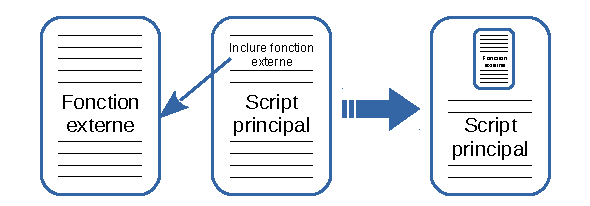
\includegraphics[scale=1.2]{images/include.pdf}

\caption{Mécanisme d'inclusion d'un fichier}
\label{inclusion}
\end{center}
\end{figure}

En effet, inclure du code contenu dans un autre fichier permet, entre autre, les deux utilisations suivantes :
\begin{itemize}
\item inclure des portions de code différentes en fonction de choix de l'utilisateur ou de l'environnement de ce dernier;
\item inclure des portions de code utilisées dans plusieurs scripts (par exemple une fonction de connexion à une base de données) afin de ne pas avoir à recopier les mêmes lignes à différents endroits et de ne modifier qu'un seul fichier en cas de modification de la fonction.
\end{itemize}


Nous voyons donc que le premier point ci-dessus permet d'obtenir une réelle adaptabilité du code alors que le second point donne la possibilité au développeur d'écrire du code concis et factorisé. Nous allons cependant voir que ce mécanisme n'est pas dépourvu de vulnérabilités.


\subsection{Description de la vulnérabilité}

La principale vulnérabilité connue dans le mécanisme que nous venons d'expliciter intervient lorsque l'inclusion d'un script est gérée par une variable pouvant être contrôlée par un attaquant. On se retrouve alors plutôt dans le premier cas d'utilisation indiqué, c'est à dire inclure des portions de code différentes en fonction de choix de l'utilisateur ou de l'environnement de ce dernier. En effet, dans le second cas d'utilisation, l'inclusion du fichier est généralement écrite "en dur" dans le script principal et ne peut donc pas être facilement modifiée par un attaquant.

\begin{figure}[!h]
\begin{center}


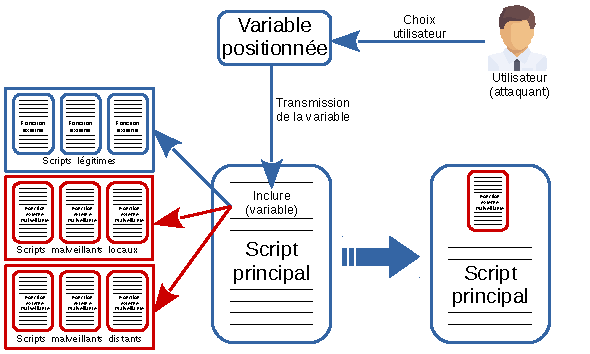
\includegraphics[scale=1.4]{images/include_hacked.pdf}

\caption{Vulnérabilité d'inclusion d'un fichier}
\label{inclusion_hacked}
\end{center}
\end{figure}

On remarque dans le schéma \ref{inclusion_hacked} que dans le cas où un attaquant peut avoir accès à la variable permettant de sélectionner le script légitime, celui-ci peut en modifier le contenu de deux façons. On parle alors de \textit{Local File Inclusion} (LFI) et de \textit{Remote File Inclusion} (RFI).

\subsubsection{Local File Inclusion}

Une fois que l'attaquant est en capacité de modifier le contenu de la variable indiquant le nom du script à inclure, celui-ci peut y indiquer un chemin local (i.e. directement sur le serveur) vers un script contenant du code malveillant. Il peut s'agir d'un script que l'attaquant a au préalable placé sur le serveur ou d'un script déjà présent qui effectue des opérations pouvant porter atteinte à la disponibilité de la machine voire à l'intégrité ou la confidentialité des données.

\subsubsection{Remote File Inclusion}

L'attaquant peut également indiquer dans la variable un chemin distant (i.e. vers un autre serveur) pointant vers un script contenant du code malveillant. Cette technique a pour avantage de faciliter la gestion du contenu du script malveillant par l'attaquant qui peut y inclure toutes les fonctionnalités qu'il souhaite voire le faire évoluer en fonction de la réponse de la machine attaquée.\\

Dans les deux cas, les scripts malveillants sont recopiés au sein du code du script principal qui sera au final exécuté par le serveur. Cette vulnérabilité offre donc de vastes possibilités à un attaquant qui peut alors faire exécuter par un serveur n'importe quelles fonctionnalités qu'il souhaite.

\subsection{Exploitation de la vulnérabilité}
\label{expl_fi}
Afin d'illustrer avec l'application DVWA la vulnérabilité d'une inclusion de fichier mal protégée, nous cherchons à lire les cinq citations incluses dans un fichier \texttt{fi.php}. Ce fichier se trouve dans le répertoire \path{dvwa/hackable/flags} de DVWA. Ces citations devront bien entendu être lues grâce à la technique de l'inclusion de fichier. 

Cette exploitation se déroulera en trois étapes et illustrera la technique du \textit{Local File Inclusion}. Une quatrième partie étendra cette exploitation au \textit{Remote File Inclusion}.

\subsubsection{Détection d'une inclusion de fichier}

La page "\textit{File Inclusion}" accessible depuis le menu de gauche de DVWA permet, notamment, d'accéder à trois pages intitulées \texttt{file1.php}, \texttt{file2.php} et \texttt{file3.php}. 

\begin{figure}[!h]
\begin{center}
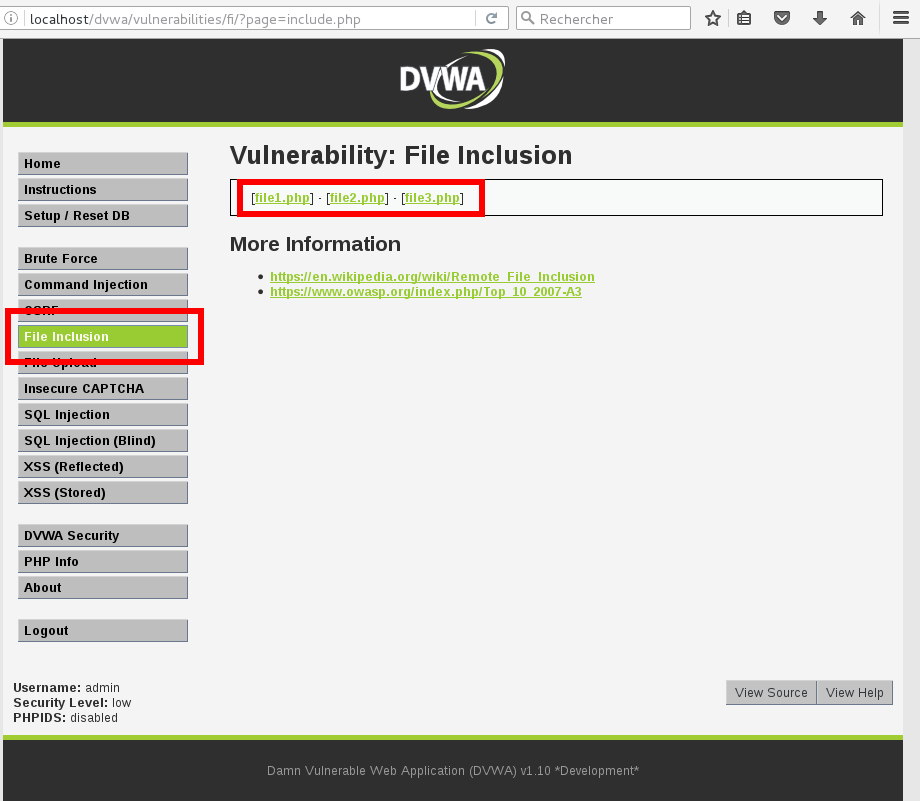
\includegraphics[scale=.34]{images/fi1.png}

\caption{Page "File Inclusion" de DVWA}
\label{fi_dvwa1}
\end{center}
\end{figure}

En cliquant par exemple sur \texttt{file1.php}, il est possible de se rendre compte que le nom du fichier est passé en paramètre de l'URL (cf. figure \ref{fi_dvwa2}). On peut alors faire l'hypothèse que la valeur du champ "\textit{page}" de l'URL est utilisée pour positionner la variable indiquant le nom du fichier à inclure par le script PHP affichant la page. 

\begin{figure}[!h]
\begin{center}
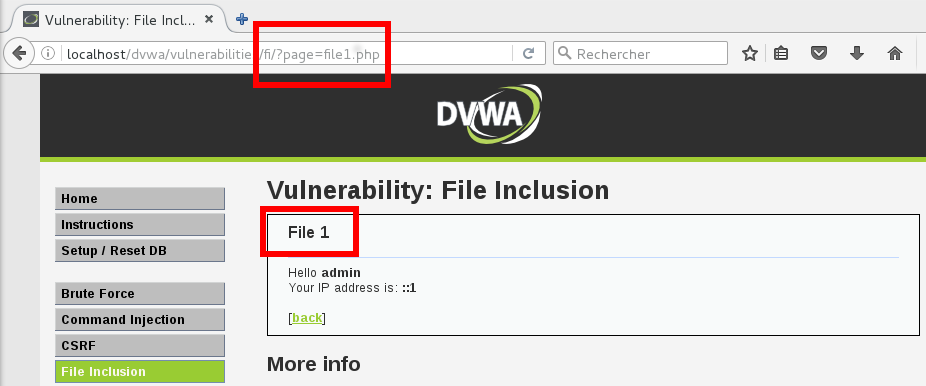
\includegraphics[scale=.5]{images/fi2.png}

\caption{Nom de la page sélectionné en paramètre de l'URL}
\label{fi_dvwa2}
\end{center}
\end{figure}

Nous venons donc très probablement de trouver un moyen d'agir sur la variable indiquant le nom du fichier à inclure. L'idée étant de lire un fichier déjà présent sur le serveur, il est nécessaire de connaitre un minimum l'arborescence de l'application web. 

\subsubsection{Connaissance de l'arborescence de l'application web}
\label{arb}

Certains sites avec une mauvaise configuration du serveur permettent de "lister" les répertoire présents sur le serveur web. Ceux-ci s'affichent alors comme dans un explorateur de fichier et la connaissance de l'arborescence de l'application est immédiate.

Dans le cas de DVWA, il n'est pas possible de connaitre directement l'arborescence entière du serveur même si certains dossiers peuvent être listés (e.g.\ \path{dvwa/vulnerabilities/}). Cependant, nous connaissons déjà l'emplacement sur le serveur du fichier que nous souhaitons exécuter : \path{dvwa/hackable/flags/fi.php}. De plus, nous savons que nous nous trouvons dans le répertoire \path{dvwa/vulnerabilities/fi/}. Ainsi, le chemin relatif pour accéder au fichier souhaité depuis la page contenant le script d'inclusion serait : \path{../../hackable/flags/fi.php}.

Dans le cadre de la technique du \textit{Local File Inclusion}, il est nécessaire et parfois difficile de connaitre l'emplacement exact du fichier que l'on souhaite exécuter dans l'arborescence de l'application. Dans le cas où, comme ici, nous n'avons pas d'affichage direct de cette arborescence, il peut être nécessaire de "tâtonner" afin d'arriver jusqu'au fichier souhaité.

Nous pouvons maintenant tenter de lire les citations auxquelles nous souhaitons accéder.

\subsubsection{Affichage et lecture du fichier}


Comme le paramètre "\textit{page}" de l'URL semble directement fournir le chemin d'inclusion du fichier au script principal, on peut tenter d'indiquer \path{../../hackable/flags/fi.php} à la place de \path{file1.php} dans l'URL.

\begin{figure}[!h]
\begin{center}
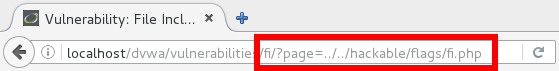
\includegraphics[scale=.6]{images/fi3.png}

\caption{Passage en paramètre du chemin vers le fichier}
\label{fi_dvwa3}
\end{center}
\end{figure}


Nous voyons alors dans la figure \ref{fi_dvwa4} que nous avons pu inclure en haut de la page courante le fichier \path{fi.php}. Les citations 1, 2 et 4 sont directement affichées. La citation 3 est masquée et la citation 5 se trouve dans les commentaires du code source du fichier HTML.

\begin{figure}[!h]
\begin{center}
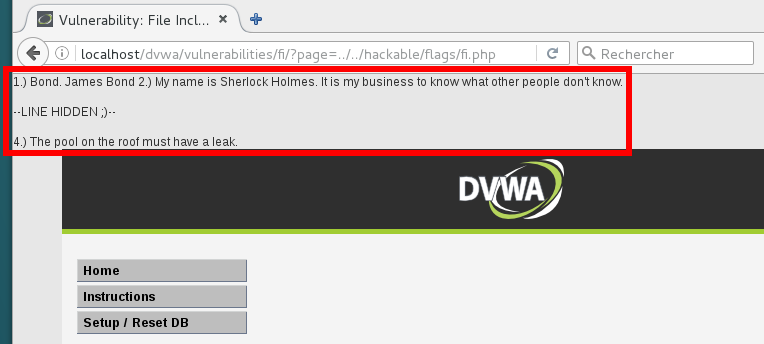
\includegraphics[scale=.6]{images/fi4.png}

\caption{Inclusion de \texttt{fi.php} dans la page principale}
\label{fi_dvwa4}
\end{center}
\end{figure}

Conformément au schéma de la figure \ref{inclusion_hacked}, nous avons, en modifiant la valeur d'une variable, redirigé le chemin du fichier à inclure dans la page courante vers le fichier de notre choix. Ce fichier \path{fi.php} est bien exécuté par le serveur. Il ne contient ici que du texte mais pourrait également contenir du code malveillant qui serait tout autant exécuté.

\subsubsection{Extension au \textit{Remote File Inclusion}}

Dans l'exemple que nous avons étudié ici, nous avons vu qu'il s'agissait d'exécuter un fichier PHP déjà présent sur le serveur. La section \ref{arb} nous a permis de trouver comment accéder localement au fichier souhaité.

Il faut cependant noter que nous pouvons appliquer une technique presque en tout point similaire pour exécuter des fichiers qui se trouvent sur un autre serveur et accessibles depuis une URL. Il s'agit de la technique du \textit{Remote File Inclusion}. Il suffit pour cela de passer en paramètre de l'argument "\textit{page}" l'adresse à laquelle un script se trouve. Là encore, le script sera exécuté par l'application sans aucune protection (cf.\ figure \ref{fi_dvwa5}).

\begin{figure}[!h]
\begin{center}
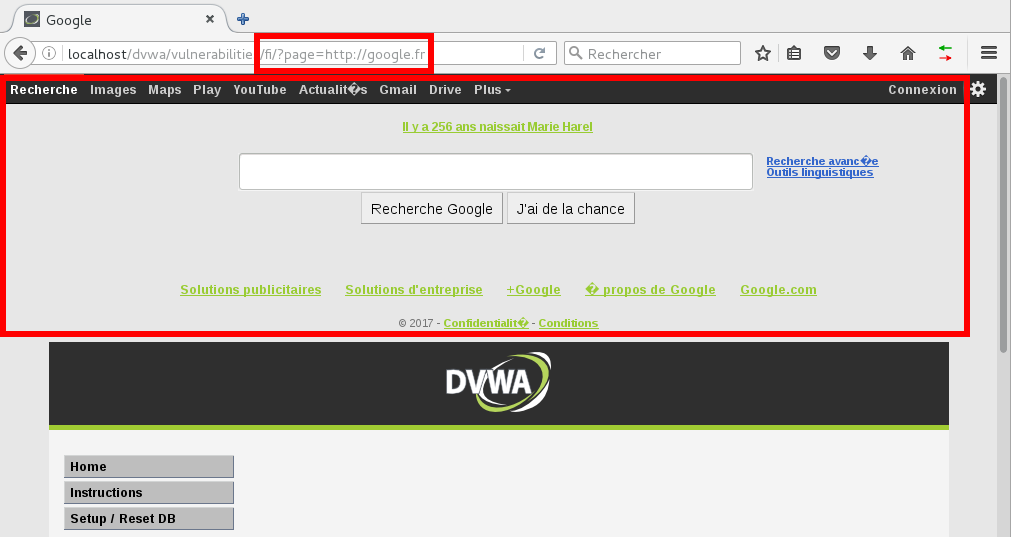
\includegraphics[scale=.45]{images/fi5.png}

\caption{Inclusion de \url{http://google.fr} dans la page principale}
\label{fi_dvwa5}
\end{center}
\end{figure}

\subsection{Contre-mesures}

L'application DVWA implémente trois niveaux de contre-mesures afin de se protéger contre la vulnérabilité explicitée ci-dessus.

\subsubsection{Premier niveau}

\paragraph{Description de l'implémentation :}

La première contre-mesure implémentée par DVWA consiste à ajouter les lignes suivantes dans le script PHP récupérant la valeur du paramètre "\textit{page}" :

\begin{lstlisting}
// Input validation
$file = str_replace( array( "http://", "https://" ), "", $file );
$file = str_replace( array( "../", "..\"" ), "", $file ); 
\end{lstlisting}

La fonction \texttt{str\_replace()} en PHP permet de rechercher dans une chaine de caractère le motif passé dans le premier argument, de le remplacer par celui passé dans le deuxième argument et d'affecter le résultat dans la variable passée en troisième argument.

Dans notre exemple, la première ligne tente de se prémunir contre la technique du \textit{Remote File Inclusion} en supprimant la mention aux protocoles HTTP et HTTPS permettant de récupérer une page ou un script présent sur un autre serveur.

La seconde ligne tente, elle, de se prémunir contre la technique du \textit{Local File Inclusion}. En effet, elle tente d'éviter tout déplacement du répertoire courant sur le serveur en supprimant les motifs du type "\texttt{../}".

\paragraph{Faiblesses de la contre-mesure :}

La contre-mesure tentant de se prémunir contre la technique du \textit{Local File Inclusion} ne permet de supprimer qu'un seul motif "../" et ne gère pas la succession potentielle de celui-ci. Ainsi, il reste possible d'atteindre le fichier souhaité sur le serveur en rajoutant simplement un motif "../" supplémentaire qui sera supprimé. On retrouvera, par là, le chemin exact vers le fichier visé.

En ce qui concerne la contre-mesure permettant de se prémunir contre la technique du \textit{Remote File Inclusion}, on peut noter que seuls les URL commençant par "\texttt{http://}" sont filtrés. Or le langage PHP est capable de gérer d'autres types de protocoles écrits dans le style URL comme "php://" qui accède à différents flux d'entrée/sortie. Par exemple, l'URL "\texttt{php://input}"\footnote{Voir documentation PHP : \url{http://php.net/manual/fr/wrappers.php.php}} est capable de lire des données brutes écrites dans le corps d'une requête POST. Ainsi, en créant nous même une requête POST dans laquelle on écrit du code PHP et que l'on envoie à l'adresse \texttt{http://localhost/dvwa/vulnerabilities/fi/?page=php://input}, il sera bien possible de faire exécuter par le serveur la portion de code incluse dans la requête. En effet, la chaine "\texttt{php://input}" passée au paramètre "\textit{page}" de l'URL ne sera pas filtrée et sera exécutée lors de son inclusion. L'interpréteur PHP ira alors lire les données écrites dans le corps de la requête POST et exécutera le code qu'il trouvera.

Afin d'illustrer ce propos, nous allons utiliser l'add-on "\href{https://addons.mozilla.org/fr/firefox/addon/hackbar/}{\textit{Hackbar}}" de Firefox qui permet, entre autre, de créer soi-même des requêtes POST.


\begin{figure}[!h]
\begin{center}
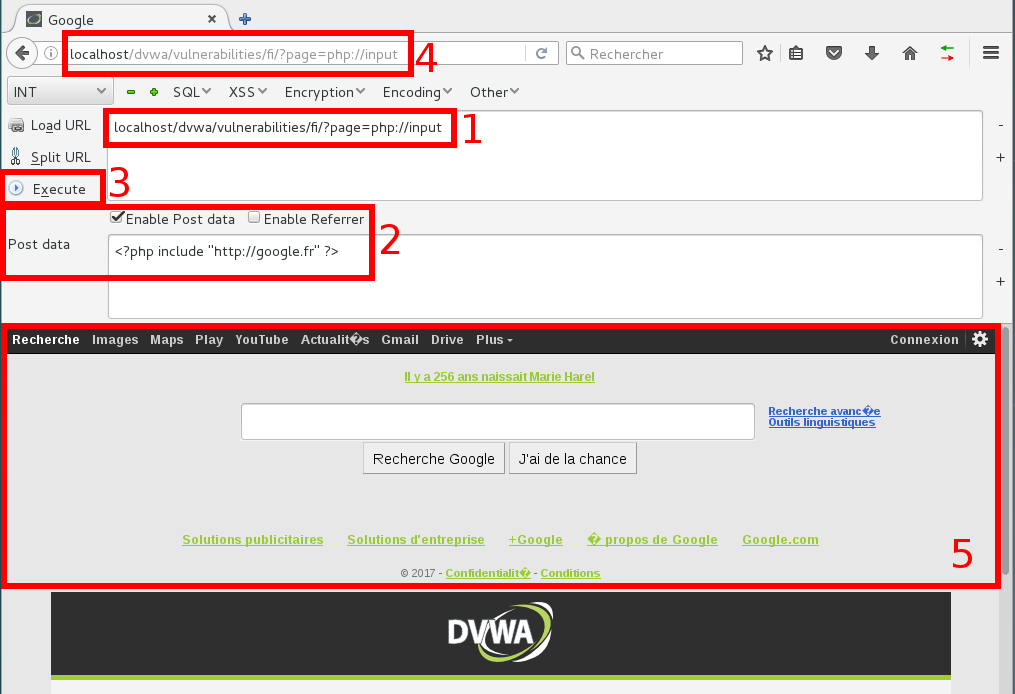
\includegraphics[scale=.41]{images/fi6.png}

\caption{Création d'une requête POST pour l'inclusion de \url{http://google.fr} dans la page principale}
\label{fi_dvwa6}
\end{center}
\end{figure}


On prévoit d'envoyer la requête POST à l'adresse \path{http://localhost/dvwa/vulnerabilities/fi/?page=php://input} (1) et on y inclus le code suivant (2) permettant l'inclusion de la page \url{http://google.fr} :
\begin{lstlisting}
<?php include "http://google.fr"; ?>
\end{lstlisting}
On exécute ensuite la requête (3) qui est transmise au navigateur (4). La page DVWA inclut bien les éléments (5) de la page \url{http://google.fr} (RFI). En effet, on vérifie bien dans la figure \ref{fi_dvwa7} que la requête POST envoyée au serveur contient la portion de code écrite. On pourrait de la même manière demander dans le code PHP l'inclusion d'un script présent sur le serveur (LFI).

\begin{figure}[!h]
\begin{center}
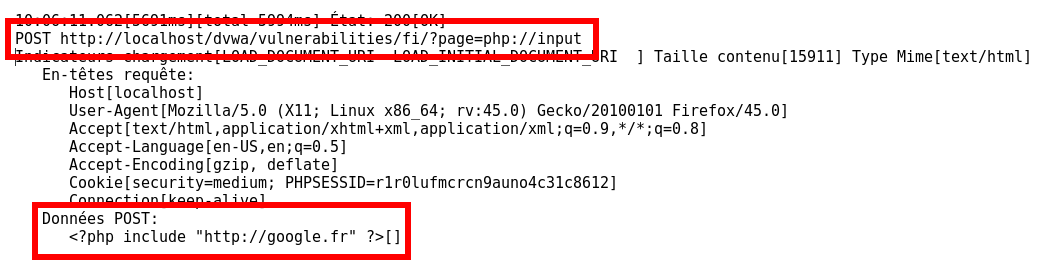
\includegraphics[scale=.45]{images/fi7.png}

\caption{Requête POST envoyée au serveur}
\label{fi_dvwa7}
\end{center}
\end{figure}

On voit donc que les protections ajoutées au code PHP ne sont pas suffisantes puisque l'on peut encore appliquer les techniques du \textit{Local File Inclusion} et du \textit{Remote File Inclusion}. Voyons maintenant de nouvelles protections proposées par DVWA.

\subsubsection{Deuxième niveau}

\paragraph{Description de l'implémentation :}


Afin de remédier aux problèmes énoncés ci-dessus, un deuxième niveau de sécurité contre l'inclusion de fichier a été implémenté dans DVWA en supprimant le code précédent et en ajoutant le test  suivant :
\begin{lstlisting}
// Input validation
if( !fnmatch( "file*", $file ) && $file != "include.php" ) {
    // This isn't the page we want!
    echo "ERROR: File not found!";
    exit;
} 
\end{lstlisting}

Le test implémenté permet de vérifier le nom du fichier passé en paramètre et s'il ne s'agit pas de \texttt{include.php} ou d'un nom commençant par "\texttt{file}", une erreur est retournée.

\paragraph{Faiblesses de la contre-mesure :}

Concernant le test de la chaine de caractère commençant par "\texttt{file}", on remarque que le test ne s'effectue que sur le début de la chaine de caractère. Il reste donc possible d'accéder à des fichiers dans le répertoire courant commençant par "\texttt{file}" et qui ne seraient en temps normal pas accessibles. 

Par exemple, un fichier \texttt{file4.php} se trouve dans le répertoire courant. Si le concepteur souhaitait que les utilisateurs n'aient pas accès à ce fichier, le test effectué à ce niveau de sécurité ne permet pas de se prémunir contre un accès non désiré. En effet, le fichier commence bien par "\texttt{file}" et aucune erreur ne sera retourné comme le montre la figure \ref{fi_dvwa8}.

\begin{figure}[!h]
\begin{center}
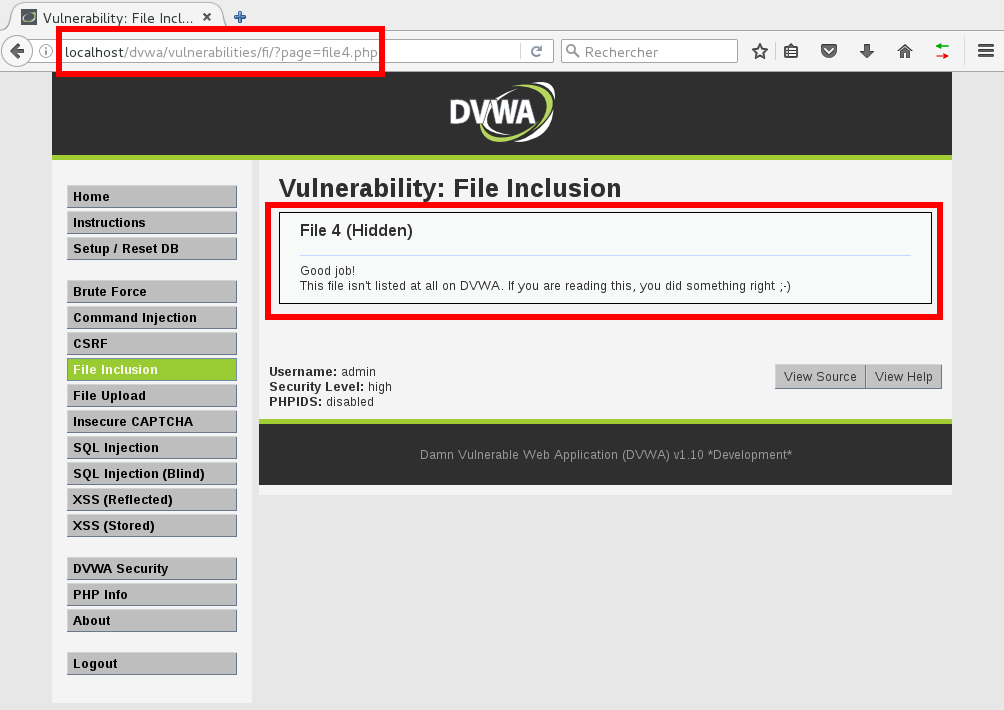
\includegraphics[scale=.45]{images/fi8.png}

\caption{Affichage de \texttt{file4.php}}
\label{fi_dvwa8}
\end{center}
\end{figure}

On peut également noter que la fonction d'inclusion de PHP (\texttt{include}) accepte en paramètre d'autres protocole que HTTP. Ainsi, il est possible d'utiliser le protocole \texttt{file} qui permet d'accéder au système de fichier. Il suffit de passer en paramètre de page \path{file://CHEMIN/VERS/LE/SCRIPT/LOCAL}. La chaine de caractère commencera bien par "\texttt{file}" et il sera ainsi possible d'accéder par la technique du \textit{Local File Inclusion} à n'importe quel script présent sur le serveur. On peut par exemple passer en paramètre de l'URL le chemin \path{file:///var/www/html/dvwa/hackable/flags/fi.php} pour accéder aux citations que l'on souhaitait afficher dans la section \ref{expl_fi}. La figure \ref{fi_dvwa9} montre bien que l'accès à ce fichier est encore possible malgré les nouveaux éléments de contrôle implémentés.\\

\begin{figure}[!h]
\begin{center}
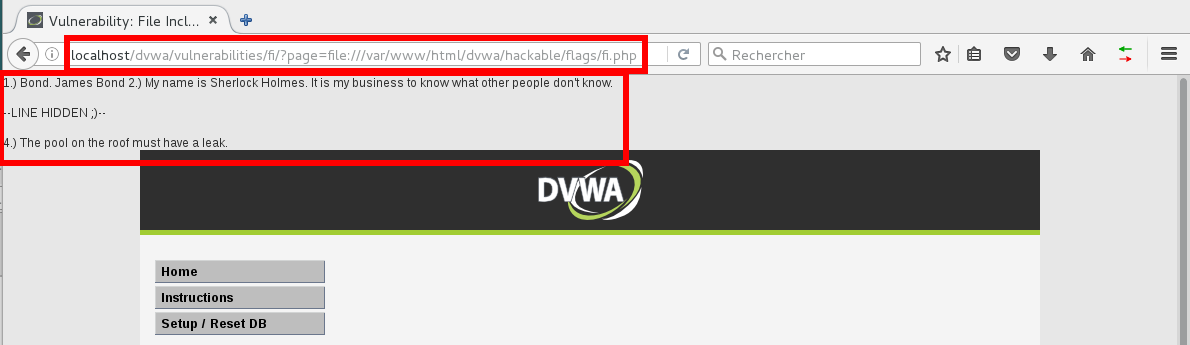
\includegraphics[scale=.4]{images/fi9.png}

\caption{Affichage des citations contenues dans \texttt{fi.php}}
\label{fi_dvwa9}
\end{center}
\end{figure}


Pour aller plus loin et comme nous le verrons dans un autre type de vulnérabilité (cf. section \ref{fu} \textit{File Upload}), si un attaquant a pu charger dans le répertoire courant un fichier commençant par "file" ou s'il a pu charger un fichier à n'importe quel endroit du serveur, celui-ci sera toujours en mesure de l'exécuter grâce à la technique du \textit{Local File Inclusion} et malgré les mesures de sécurité mises en place. On remarque cependant que la technique du \textit{Remote File Inclusion} semble mise à mal à ce niveau de sécurité et que la seule façon d'inclure du code distant est de se servir d'un script local placé grâce à une vulnérabilité dans le chargement de fichier par exemple. Comme il sera de toute façon nécessaire de faire appel à ce fichier local pour accéder au code distant, on se retrouve plutôt dans une technique de \textit{Local File Inclusion}. 

Voyons maintenant comment est-il possible de faire face aux vulnérabilités encore présentes.

\subsubsection{Troisième niveau}

\paragraph{Description de l'implémentation :}

Une dernière implémentation dans l'application DVWA remplace le test précédent par celui qui suit :

\begin{lstlisting}
// Only allow include.php or file{1..3}.php
if( $file != "include.php" && $file != "file1.php" && $file != "file2.php" && 
    $file != "file3.php" ) {
    // This isn't the page we want!
    echo "ERROR: File not found!";
    exit;
}
\end{lstlisting}

On remarque que le test effectue une vérification exhaustive du nom des fichiers accessibles. Ainsi, toute chaine de caractères passée en paramètre de l'URL qui ne correspondrait pas à l'un des quatre nom énuméré retournera une erreur.

\paragraph{Faiblesses de la contre-mesure :}

Une telle implémentation se trouve apparemment dépourvue de faiblesse en ce qui concerne la chaine de caractères passé en paramètre de l'URL. Cependant, cette protection peut encore être détournée par le chargement d'un fichier qui viendrait écraser un ficher au nom légitime. On se retrouverait alors avec un fichier dont le nom correspondrait bien à l'un de ceux énuméré mais qui contiendrait du code malicieux. 

La section suivante s'attache à analyser les différentes façons de se prémunir contre ce type de vulnérabilité.


\section{File Upload}
\label{fu}

De très nombreuses applications web laissent la possibilité à l'utilisateur de charger sur le serveur des fichiers qu'il détient en local sur son propre ordinateur. On peut bien entendu citer à ce titre les serveurs de messagerie électronique ainsi que les clients web permettant la gestion d'un \textit{cloud}. En effet, sans cette fonctionnalité de chargement, il serait impossible de joindre un fichier à mail ou même de sauvegarder ses fichiers dans le \textit{cloud}. 

Nous allons voir que cette fonctionnalité doit être bien encadrée et supervisée afin de ne pas créer de très importantes vulnérabilités.

\subsection{Description de la vulnérabilité}

\subsubsection{Généralités}

Le chargement d'un fichier local vers un serveur web est une fonctionnalité nécessaire voire inhérente à certaines applications web. Sans cette possibilité, certaines applications n'auraient même pas de raison d'être. Ainsi, \textit{Gmail}, \textit{Google Drive} ou \textit{DropBox} reposent sur cette possibilité. Il est donc nécessaire de trouver le moyen de faire face aux différentes vulnérabilités de cette fonction.

Un grand nombre d'attaques sur les applications web se déroulent en deux phases :
\begin{enumerate}
\item injection d'un code malicieux sur le serveur web;
\item exécution du code malicieux précédemment injecté.
\end{enumerate} 
On peut donc clairement voir que le chargement d'un fichier local vers un serveur web offre la possibilité à un attaquant d'introduire sur le serveur web un fichier contenant du code malicieux. Il ne lui restera alors plus qu'à trouver un moyen d'exécuter ce code comme nous avons pu le voir dans section \ref{fi}.

De plus, il est à noter que n'importe quel type de script peut, grâce à cette fonction, être importé sur le serveur web. Cela laisse donc la porte ouverte à un grand nombre d'attaques différentes : déni de service, défacement, prise en main du système, etc...

Afin de retirer ces possibilités d'action à un attaquant éventuel, il sera nécessaire de restreindre le chargement à certains types de fichiers ou d'effectuer certains contrôles.

\subsubsection{Différentes vulnérabilités}

La plateforme \href{http://www.owasp.org}{OWASP} classe les vulnérabilités liées au chargement de fichiers en deux catégories : les vulnérabilités liées aux méta-données et les vulnérabilités liées à la taille ou au type des fichier.

\paragraph{Les vulnérabilités liées aux méta-données :}

Ces vulnérabilités sont dues aux différents champs échangés dans les requêtes HTTP, principalement le champ indiquant le chemin de destination du fichier ainsi que le champ indiquant le nom du fichier.

En effet, en modifiant les champs des requêtes HTTP \textit{multi-part} (utilisées dans le chargement et le téléchargement de fichiers sur un serveur web), il est possible d'écraser des fichiers déjà existants ou même d'atteindre des répertoires normalement non autorisés à l'écriture par un utilisateur.

Cette classe de vulnérabilités permet donc, par exemple, d'effectuer un défacement, d'insérer du code malicieux dans des dossiers stratégiques ou encore de modifier le comportement normal d'un script.

\paragraph{Les vulnérabilités liées à la taille ou au type des fichiers :}

Ces vulnérabilités sont principalement dues à l'absence de certaines vérifications avant le début du chargement du fichier. 

Ainsi, la non vérification de la taille d'un fichier laisse la possibilité aux utilisateurs de charger des fichiers aussi volumineux qu'ils le souhaitent. Il est alors possible sur certains serveurs dont l'espace de stockage est limité d'atteindre la capacité maximale de cet espace et, par là, de rendre la fonctionnalité de chargement voire le serveur lui-même indisponible. On peut donc aboutir très rapidement à une attaque du type déni de service.

De même, la non-vérification du type de fichier peut permettre à un utilisateur de charger sur le serveur un script exécutable alors que le fichier attendu était par exemple une simple photographie. Un tel script pourra alors être \textit{a posteriori} exécuté par l'attaquant, lui donnant ainsi de nombreuses possibilités.\\

On voit donc que le chargement de fichier sur un serveur web est loin d'être anodin et doit être encadré afin d'éviter qu'un utilisateur ait à sa disposition un large éventail d'attaques possibles.


\subsection{Exploitation de la vulnérabilité}

Afin d'illustrer la vulnérabilité d'un chargement de fichier non sécurisé, la page "\textit{File Upload}" accessible depuis le menu de gauche de DVWA propose une interface permettant le chargement sur le serveur d'un fichier local. Le texte du formulaire nous indique qu'une image est attendue mais nous allons voir que d'autres types de fichiers peuvent également être acceptés.

\subsubsection{Chargement du fichier}

Nous allons créer en local un fichier \texttt{fu.php} contenant les trois lignes de code suivantes :

\begin{lstlisting}
<?php
  phpinfo();
?>
\end{lstlisting}

L'idée est simplement ici de faire exécuter du code PHP que l'on a introduit sur le serveur par l'intermédiaire du chargement de fichier. Dans le cas présent, la fonction \texttt{phpinfo()} affiche les éléments de configuration de l'environnement PHP du serveur.

On sélectionne donc notre fichier \texttt{fu.php} à partir du formulaire de la page "File Upload" et l'application nous indique "\texttt{../../hackable/uploads/fu.php succesfully uploaded!}" comme le montre la figure \ref{fu_dvwa1}.

\begin{figure}[!h]
\begin{center}
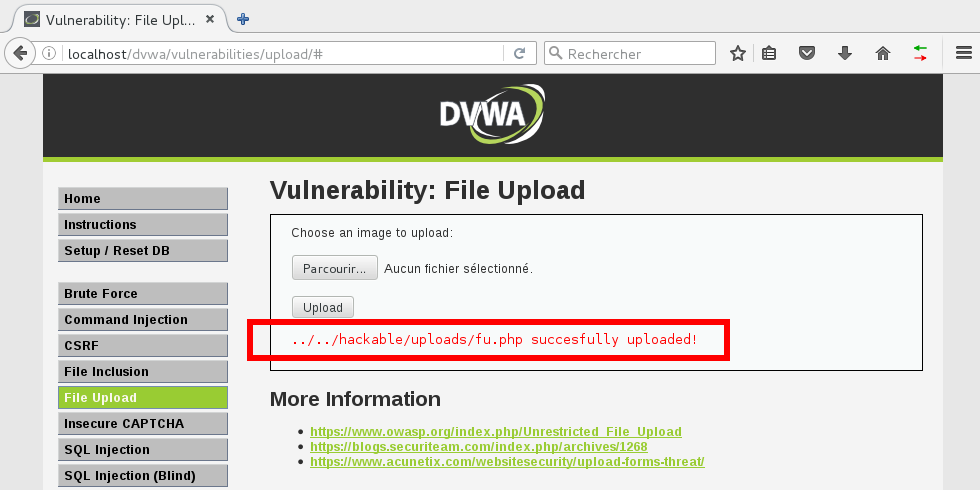
\includegraphics[scale=.45]{images/fu1.png}

\caption{Chargement réussi du script \texttt{fu.php}}
\label{fu_dvwa1}
\end{center}
\end{figure}


\subsubsection{Exécution du script}

Nous voyons dans la figure \ref{fu_dvwa1} que DVWA nous indique clairement dans quel répertoire (relatif) se trouve le fichier. Il suffit maintenant de saisir dans le navigateur l'adresse \path{http://localhost/dvwa/hackable/uploads/fu.php} et le fichier que nous avons créé est bien exécuté sur le serveur comme le montre la figure \ref{fu_dvwa2}.

\begin{figure}[!h]
\begin{center}
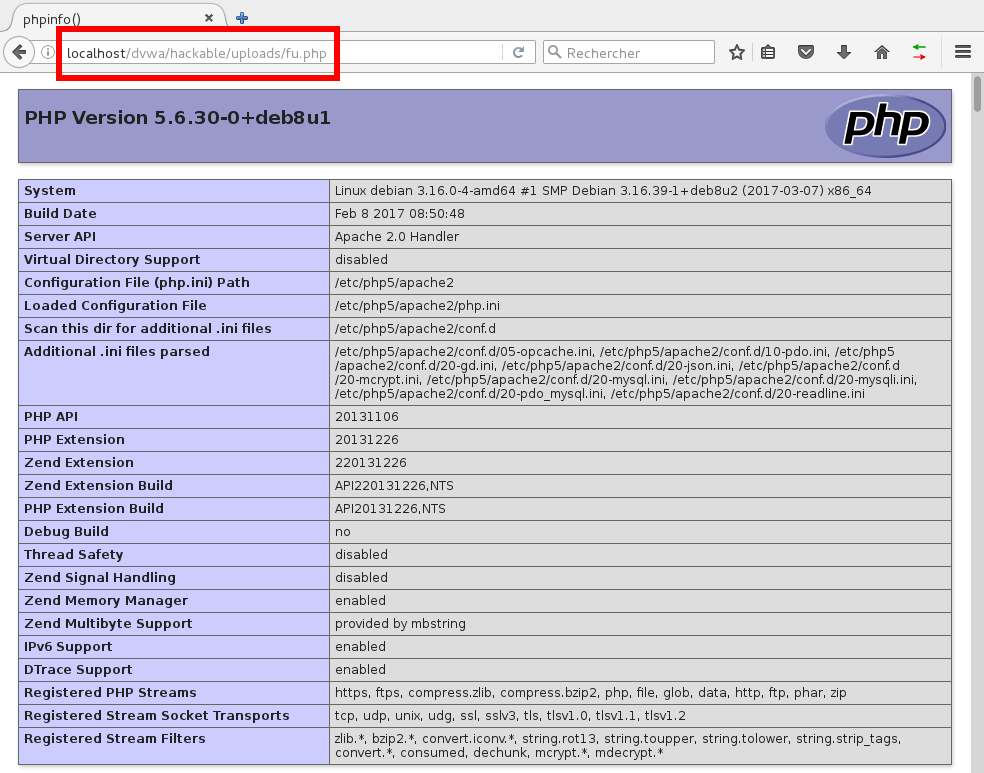
\includegraphics[scale=.45]{images/fu2.png}

\caption{Exécution du script \texttt{fu.php}}
\label{fu_dvwa2}
\end{center}
\end{figure}

Il est à noter ici que nous ne faisons qu'afficher la configuration de l'environnement PHP mais il serait également possible d'exécuter n'importe quelles fonctions PHP comme des appels système. On voit donc clairement qu'un chargement de fichier non sécurisé peut constituer un réel danger pour le serveur. Voyons quelques contre-mesures permettant de se protéger contre ce type d'attaque.



\subsection{Contre-mesures}

L'application DVWA propose trois niveaux de contre-mesures afin de se protéger contre la vulnérabilité explicitée ci-dessus.

\subsubsection{Premier niveau}


\paragraph{Description de l'implémentation :}

Le premier niveau de sécurité implémenté par DVWA tente de s'assurer que le fichier chargé est bien une image. Pour cela, le test suivant est effectué avant tout traitement du fichier :

\begin{lstlisting}
// File information
$uploaded_name = $_FILES[ 'uploaded' ][ 'name' ];
$uploaded_type = $_FILES[ 'uploaded' ][ 'type' ];
$uploaded_size = $_FILES[ 'uploaded' ][ 'size' ];

// Is it an image? 
if( ( $uploaded_type == "image/jpeg" || $uploaded_type == "image/png" ) && 
        ( $uploaded_size < 100000 ) ) { 
        //Traitement de l'image
}
\end{lstlisting}

On voit que les données liées au fichier et envoyées par le formulaire sont stockées dans des variables, notamment le type de fichier chargé qui est stocké dans \texttt{\$uploaded\_type}. C'est justement la valeur de cette variable qui est testée pour s'assurer que le fichier envoyé est bien une image.

\paragraph{Faiblesses de la contre-mesure :}

Comme nous venons de le dire, les données testées sont à l'origine envoyées par le formulaire permettant le chargement du fichier.

Il est alors possible d'intercepter la requête POST envoyée au serveur lors de la validation du formulaire. On remarque sur la figure \ref{fu_dvwa3} présentant justement le détail de cette requête POST qu'il existe un champ POSTDATA contenant des informations comme le nom du fichier, son type et même son contenu sous forme de texte.

\begin{figure}[!h]
\begin{center}
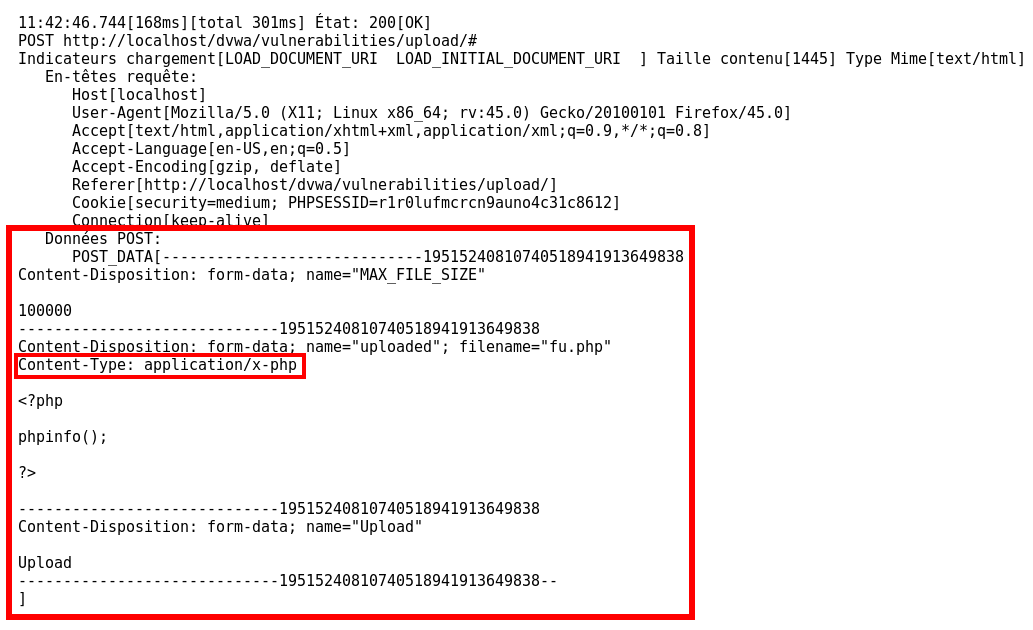
\includegraphics[scale=.45]{images/fu3.png}

\caption{Détail de la requête POST envoyée au serveur}
\label{fu_dvwa3}
\end{center}
\end{figure}

Si l'on charge une image \texttt{jpeg} ou \texttt{png}, on retrouvera bien dans le champ POSTDATA de la requête : \texttt{Content-Type: image/png}. C'est justement ces informations qui seront stockées dans la variable \texttt{\$uploaded\_type} et qui seront testées par le script.

L'idée est alors d'intercepter et modifier la requête POST envoyée au serveur lors du chargement d'un script qui n'est donc pas une image. Il est possible de modifier les informations véhiculées par la requête en y indiquant par exemple : "\texttt{Content-Type: image/png}" à la place de "\texttt{Content-Type: application/x-php}". C'est cette information qui sera stockée dans la variable \texttt{\$uploaded\_type} et le test indiquera bien qu'il s'agit d'une photo alors qu'il s'agit en fait d'un script.

Afin d'illustrer ce propos, nous allons utiliser l'add-on "\href{https://addons.mozilla.org/fr/firefox/addon/tamper-data/}{\textit{Temper Data}}" de Firefox qui permet notamment d'intercepter et de modifier les requêtes envoyées au serveur web. La figure \ref{fu_dvwa4} montre la fenêtre permettant d'altérer la requête POST envoyée au serveur. On remarque bien que l'on modifie le champ \texttt{Content-Type}.

\begin{figure}[!h]
\begin{center}
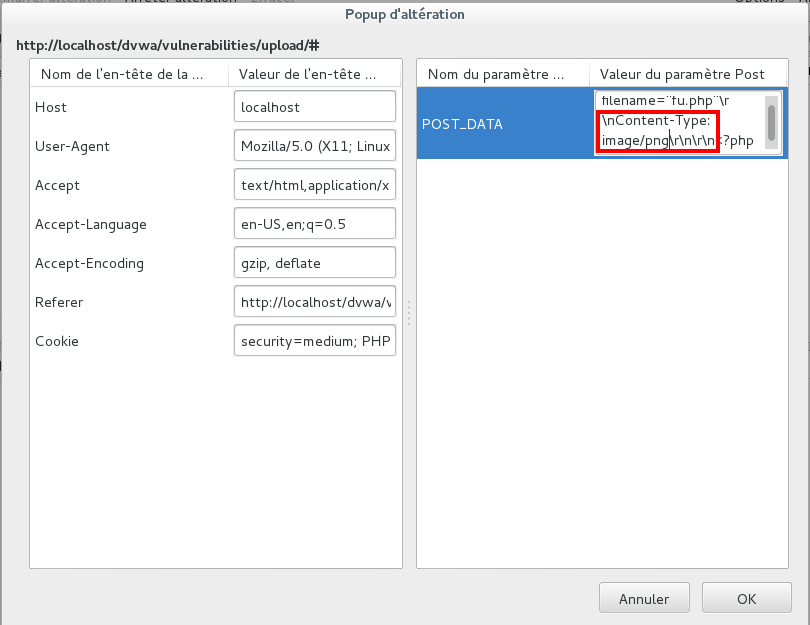
\includegraphics[scale=.45]{images/fu4.png}

\caption{Interception et modification de la requête POST}
\label{fu_dvwa4}
\end{center}
\end{figure}

Une fois la requête modifiée envoyée au serveur, on peut voir sur la figure \ref{fu_dvwa5} que DVWA nous indique bien que le fichier \texttt{fu.php} a été chargé avec succès.

\begin{figure}[!h]
\begin{center}
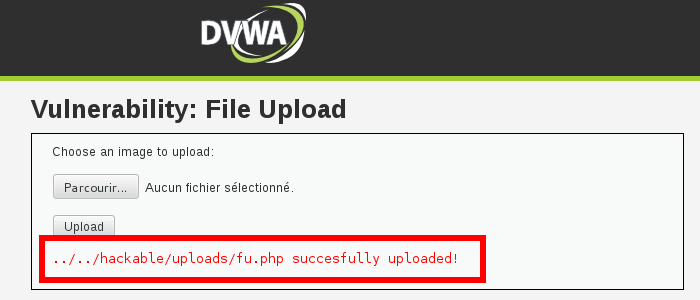
\includegraphics[scale=.45]{images/fu5.png}

\caption{Chargement avec succès de \texttt{fu.php}}
\label{fu_dvwa5}
\end{center}
\end{figure}

Il est donc possible de contourner la première protection mise en place par DVWA sur le type du fichier chargé. Un deuxième niveau de sécurité implémenté va permettre de sécuriser cette vulnérabilité.


\subsubsection{Deuxième niveau}

\paragraph{Description de l'implémentation :}

Le deuxième niveau de sécurité implémenté par DVWA effectue le test ci-dessous avant tout traitement préalable du fichier chargé :


\begin{lstlisting}
// File information
$uploaded_name = $_FILES[ 'uploaded' ][ 'name' ];
$uploaded_ext  = substr( $uploaded_name, strrpos( $uploaded_name, '.' ) + 1);
$uploaded_size = $_FILES[ 'uploaded' ][ 'size' ];
$uploaded_tmp  = $_FILES[ 'uploaded' ][ 'tmp_name' ];

// Is it an image?
if( ( strtolower( $uploaded_ext ) == "jpg" || strtolower( $uploaded_ext ) == "jpeg" || 
      strtolower( $uploaded_ext ) == "png" ) && ( $uploaded_size < 100000 ) &&
      getimagesize( $uploaded_tmp ) ) {
        //Traitement de l'image
}
        
\end{lstlisting}

On remarque qu'un traitement est tout d'abord effectué sur la chaine de caractère du nom du fichier pour en extraire seulement son extension. Celle-ci est ensuite stockée dans la variable \texttt{\$uploaded\_ext}. On teste ensuite la valeur de cette variable en s'assurant qu'il s'agit d'un fichier \texttt{jpg}, \texttt{jpeg} ou \texttt{png}. On tente également d'obtenir la taille de l'image grâce à la fonction PHP \texttt{getimagesize()}.

Ce simple test a tout d'abord l'avantage de s'assurer de l'extension réelle du fichier chargé. En effet, dans le premier niveau de sécurité, nous avions pu charger un script PHP (extension \texttt{php}) en faisant croire au serveur qu'il s'agissait d'une image. Cette technique permet d'être sûr de la façon dont sera exécuté le fichier. En effet, si l'on charge un script PHP avec l'extension d'un fichier image, le serveur traitera le fichier comme une image du fait de son extension et non comme un script PHP. Il s'agit d'une protection plutôt efficace de l'exécution des différents types de fichiers.

Ensuite, on tente également d'appliquer au fichier une fonction PHP censée fonctionner sur des fichiers de type image. Cette fonction doit permettre de retourner \texttt{False} si le fichier passé en paramètre n'est pas une image.

\paragraph{Faiblesses de la contre-mesure :}

Il est possible de faire appel à d'autres vulnérabilités pour outre-passer la protection que nous venons d'expliciter.

Il faut tout d'abord faire en sorte que la fonction PHP \texttt{getimagesize()} retourne \texttt{True} pour que le téléchargement vers le serveur ait lieu. Pour cela, il est possible d'écrire "\texttt{GIF98}" en tout début de fichier pour faire croire à la fonction qu'il s'agit d'une image \textit{GIF} (\textit{Graphics Interchange Format}). La fonction retournera alors bien la valeur \texttt{True} pour le test réalisé. De plus, nous venons de voir qu'à ce niveau de sécurité, nous pouvions charger n'importe quel fichier du moment que l'extension soit \texttt{png}, \texttt{jpg} ou \texttt{jpeg}. Une fois le test passé et le fichier chargé sur le serveur, il ne restera qu'à trouver un moyen d'exécuter ce code malgré le fait que le serveur ne reconnaitra ce fichier que comme une image.

Pour faire face à ce dernier problème, nous pouvons alors faire appel aux vulnérabilités explicitées dans la section \ref{fi} \textit{File Inclusion}. Nous avions vu qu'il restait possible, même au deuxième niveau de sécurité, d'appliquer la technique du \textit{Local File Inclusion}. Ainsi, nous pouvons charger sans aucun problème un fichier \texttt{fu.png} (cf. figure \ref{fu_dvwa6}) qui n'est autre que le fichier \texttt{fu.php} dont l'extension a été modifié et auquel a été rajouté la mention "\texttt{GIF98}" en tout début de fichier. Le fichier est alors chargé sur le serveur (cf. figure \ref{fu_dvwa6}) et il ne reste plus qu'à l'exécuter grâce à la technique du \textit{Local File Inclusion}.

\begin{figure}[!h]
\begin{center}
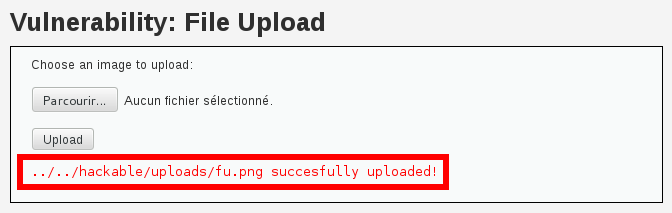
\includegraphics[scale=.5]{images/fu6.png}

\caption{Chargement avec succès de \texttt{fu.png}}
\label{fu_dvwa6}
\end{center}
\end{figure}

Pour cela, nous pouvons nous servir de la page de DVWA dédiée à la technique du \textit{Local File Inclusion} dans laquelle nous pouvons passer la chaine \texttt{file:///var/www/html/dvwa/hackable/uploads/fu.png} au paramètre "\textit{page}" de l'URL. L'inclusion du fichier ne se souciera pas de l'extension et exécutera le code comme nous pouvons le voir sur la figure \ref{fu_dvwa7} ci-dessous :

\begin{figure}[!h]
\begin{center}
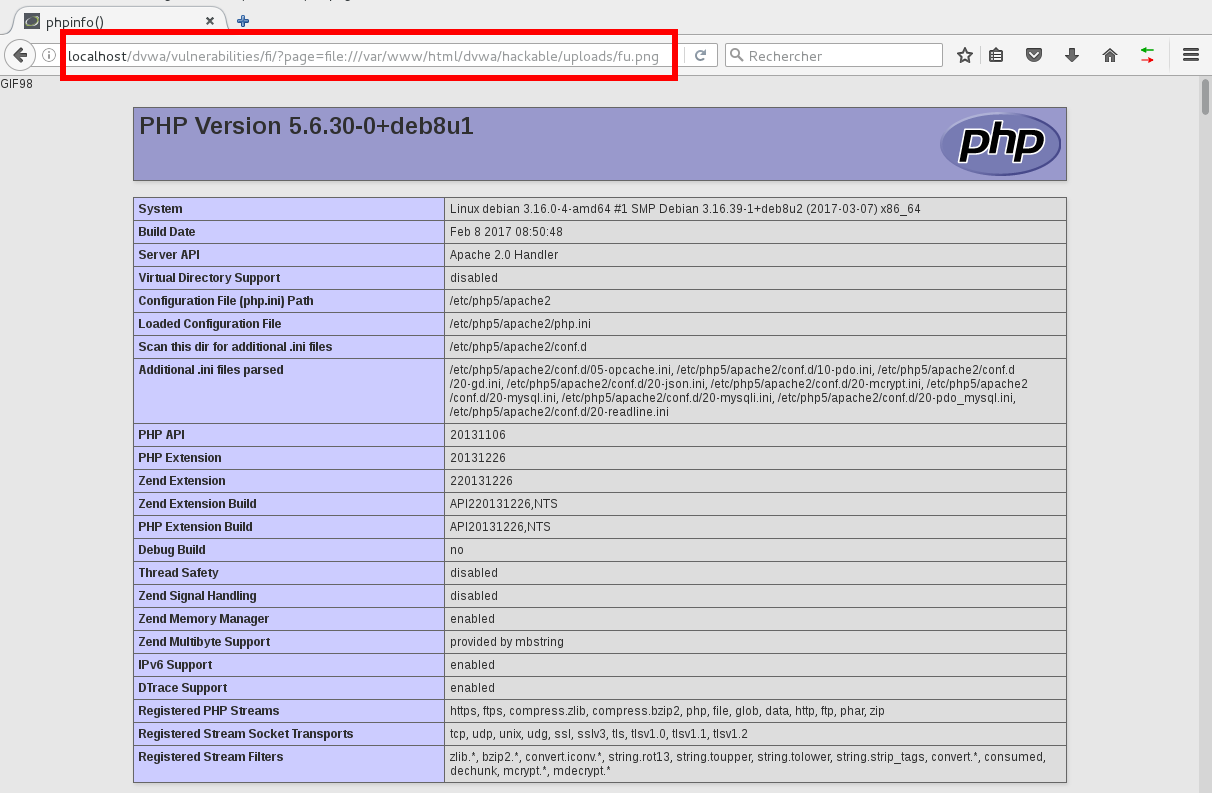
\includegraphics[scale=.35]{images/fu7.png}

\caption{Exécution avec succès du code contenu dans \texttt{fu.png}}
\label{fu_dvwa7}
\end{center}
\end{figure}

\subsubsection{Troisième niveau}

Le troisième niveau de sécurité implémenté par DVWA reprend le test du niveau précédent et, en cas de succès, exécute les lignes de code suivantes :

\begin{lstlisting}
// Strip any metadata, by re-encoding image 
// (Note, using php-Imagick is recommended over php-GD)
if( $uploaded_type == 'image/jpeg' ) {
  $img = imagecreatefromjpeg( $uploaded_tmp );
  imagejpeg( $img, $temp_file, 100);
}
else {
  $img = imagecreatefrompng( $uploaded_tmp );
  imagepng( $img, $temp_file, 9);
}
imagedestroy( $img );

// Can we move the file to the web root from the temp folder?
if( rename( $temp_file, 
    ( getcwd() . DIRECTORY_SEPARATOR . $target_path . $target_file ) ) ) {
  // Yes!
}
else {
  // No
}

// Delete any temp files
if( file_exists( $temp_file ) )
unlink( $temp_file ); 
        
\end{lstlisting}

La première partie du code ci-dessus crée une nouvelle image à partir du fichier chargé (fonctions \texttt{imagecreatefromjpeg()} et \texttt{imagecreatefrompng()}) et l'enregistre dans la variable \texttt{\$temp\_file}. Cette opération a pour but dépouiller le fichier de tout code ne correspondant pas à une image et notamment les meta-données. Cela permet donc de contrer la faiblesse explicitée dans la contre-mesure précédente.

La deuxième partie du code a, elle, pour but de déplacer le fichier au bon endroit sur le serveur. La troisième partie du code supprime tous les fichiers temporaires qui auraient pu être créés. Ces deux dernières parties permettent de se prémunir contre la présence de fichiers qui n'auraient pas été traités correctement et qui pourraient être exécutés grâce à la technique du \textit{Remote File Inclusion}.\\

L'ensemble des tests effectués à ce niveau de sécurité permettent donc de se prémunir au maximum contre le chargement de fichiers non désirés. En effet, les portions de code qui auraient notamment pu être associées à une image ne doivent pas subsister à l'issu du traitement par les fonctions PHP \texttt{imagecreatefromjpeg()} et \texttt{imagecreatefrompng()}.

\section{Insecure CAPTCHA}

De nombreux robots (ou \textit{bots}) agissent de façon automatique sur internet afin, principalement, d'envoyer des messages, qu'ils soient publicitaires ou malveillants. La plupart des spams échangés sur internet sont d'ailleurs le fait de tels robots. Il est donc nécessaire, dans certaines applications web permettant notamment l'envoi de messages, de vérifier s'il s'agit d'un humain ou d'une machine qui souhaite effectuer cette opération.

C'est dans ce but que les contrôles CAPTCHA ont été créés. En effet, CAPTCHA est l'acronyme de \textit{Completely Automated Public Turing test to tell Computers and Human Apart}. Comme son nom l'indique, ce test est censé permettre de confirmer ou non la présence d'un humain derrière la machine souhaitant réaliser une certaine opération. Ce test peut prendre plusieurs formes : reconnaissance de caractères déformés (cf. figure \ref{captcha1} ou encore reconnaissance d'éléments dans un puzzle.

\begin{figure}[!h]
\begin{center}

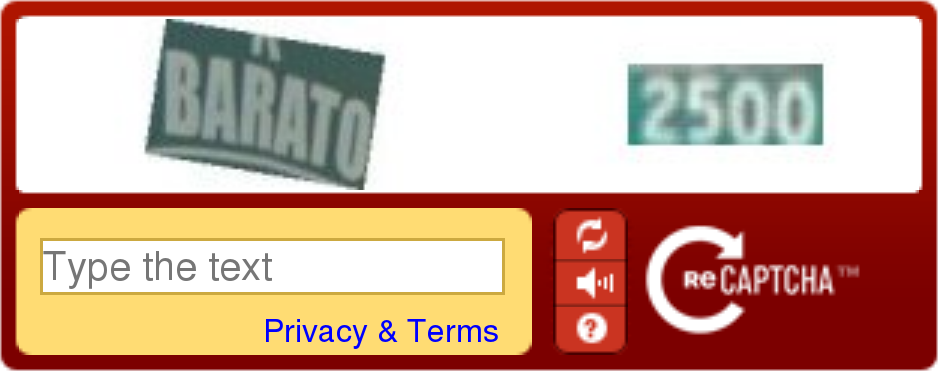
\includegraphics[scale=0.3]{images/captcha1.png}

\caption{Exemple de contrôle CAPTCHA}
\label{captcha1}
\end{center}
\end{figure}

Pour que ce test soit efficace, il est nécessaire qu'il soit implémenté de façon correcte et, ainsi, ne pas laisser la possibilité à un attaquant d'exploiter une faille qu'il pourra par la suite réutiliser dans un script automatique.
 

\subsection{Description de la vulnérabilité}
\label{desc_vul}

Différentes catégories de vulnérabilités peuvent être mises en évidence concernant les contrôles CAPTCHA.

\paragraph{Transmission de la solution :}

La première et la plus simple à exploiter est lorsque la solution se trouve être transmise en texte clair au navigateur client. Il ne suffit que de repérer l'endroit où se trouve la solution pour réaliser un script qui résoudra à coup sûr chaque contrôle CAPTCHA. En effet, les solutions peuvent être passées en argument de l'URL, dans le nom de l'image, dans un champ caché d'un formulaire HTML ou encore en commentaire du fichier HTML chargé. 

\paragraph{Mauvaise vérification de la réussite au test :}

La deuxième catégorie de vulnérabilités concerne le fait que le contrôle CAPTCHA peut être outrepassé si la vérification de la réussite au test n'est pas suffisamment sécurisée. En effet, la ou les variables indiquant une réussite ou non au test doivent être protégées et ne pas être facilement modifiées sans avoir à réaliser le test au préalable. Dans le cas contraire, il est encore possible de trouver une parade à la réalisation du test par un humain et de l'implémenter dans un script automatique.

\paragraph{Résolution automatique :}

Enfin, la troisième catégorie de vulnérabilités concerne la possibilité de résoudre de façon automatique les contrôles CAPTCHA. Dans cette catégorie, beaucoup de problèmes sont à prendre en compte : la difficulté du problème, le temps de résolution du problème ou encore l'étendue de la base de données CAPTCHA. En effet, ce dernier point est important car si la base de données d'images, par exemple, n'est pas assez grande, une entité pourrait facilement trouver un avantage financier à payer des personnes pour résoudre tous les problèmes CAPTCHA afin de pouvoir les exploiter automatiquement par la suite.

\subsection{Exploitation de la vulnérabilité}
\label{vul_captcha}

Afin d'illustrer une vulnérabilité permettant d'outre-passer un contrôle CAPTCHA, la page "\textit{Insecure CAPTCHA}" accessible depuis le menu de gauche de DVWA propose un formulaire de changement de mot de passe dont la validation est soumise à la résolution d'un contrôle CAPTCHA. Le but recherché est de modifier le mot de passe sans résoudre le contrôle CAPTCHA afin de pouvoir automatiser cette action.

Le changement de mot de passe se déroule, ici, en trois phases : 
\begin{itemize}
\item première page : double saisie du nouveau mot de passe et résolution du contrôle CAPTCHA;
\item deuxième page : vérification de la réussite au test et, en cas de succès, possibilité de valider le changement de mot de passe;
\item troisième page : vérification de la cohérence des deux mots de passe et affichage du résultat (mot de passe modifié ou non).
\end{itemize}

On remarque donc que le changement de mot de passe s'effectue réellement lors du passage de la deuxième à la troisième page. En analysant grâce à l'add-on "\href{https://addons.mozilla.org/fr/firefox/addon/tamper-data/}{\textit{Temper Data}}" de Firefox les données attendues par la requête POST entre ces deux pages, on remarque qu'elles sont au nombre de quatre (cf. figure \ref{captcha2}) : "\textit{step}", "\textit{password\_new}", "\textit{password\_conf}" et "\textit{change}"

\begin{figure}[!h]
\begin{center}


\includegraphics[scale=0.6]{images/captcha2.png}

\caption{Données attendues par la requête POST}
\label{captcha2}
\end{center}
\end{figure}

Or on peut remarquer en analysant la requête POST entre la première et la deuxième page que ces quatre données sont également attendues. On peut alors tenter de créer une requête POST dès la première page qui inclue les données normalement attendues entre la deuxième et la troisième page. On utilise pour cela l'add-on "\href{https://addons.mozilla.org/fr/firefox/addon/hackbar/}{\textit{Hackbar}}" de Firefox. La figure \ref{captcha3} montre que le changement de mot de passe est alors immédiat à partir de la première page et, cela, sans résoudre le contrôle CAPTCHA.


\begin{figure}[!h]
\begin{center}

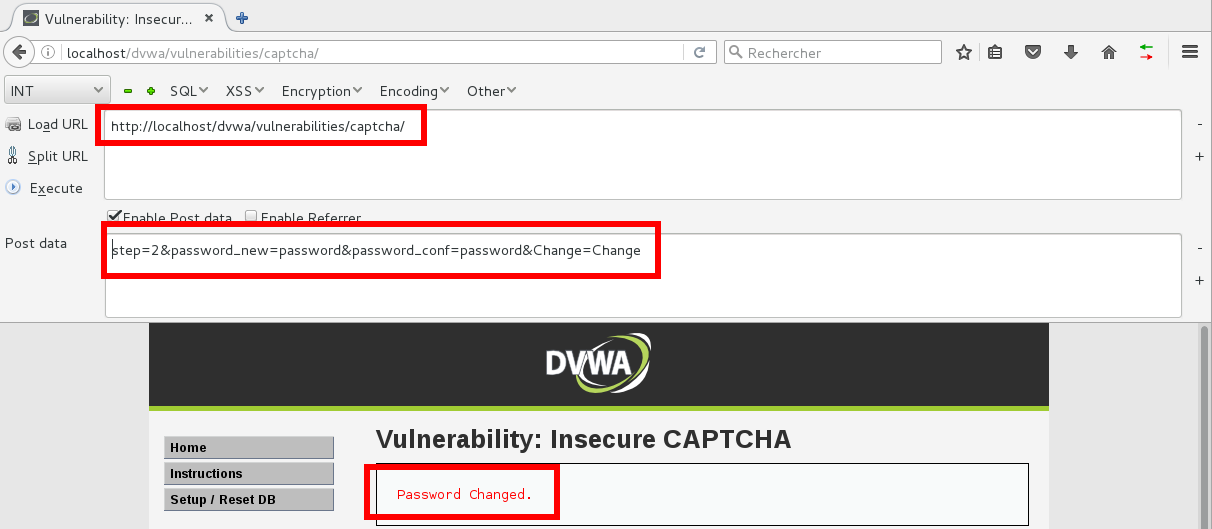
\includegraphics[scale=0.4]{images/captcha3.png}

\caption{Requête POST modifiant directement le mot de passe}
\label{captcha3}
\end{center}
\end{figure}


On voit donc qu'il est possible d'automatiser cette procédure de changement de mot de passe en créant une requête POST avec les bons paramètres. Le contrôle CAPTCHA peut ici être facilement outre-passé. Il est donc nécessaire de voir quelles contre-mesures peuvent être prises afin de garder toute l'efficacité de ce test. 

\subsection{Contre-mesures}

L'application DVWA propose trois niveaux de contre-mesures afin de se protéger contre la vulnérabilité explicitée ci-dessus.

\subsubsection{Premier niveau}

\paragraph{Description de l'implémentation :}

Nous avons pu voir dans l'exploitation de la vulnérabilité (section \ref{vul_captcha}) que la troisième page dans laquelle le mot de passe était réellement modifié pouvait être directement accessible à partir de la première page. L'idée mise en œuvre pour se prémunir de cet accès non désiré est de créer une nouvelle variable d'état dans la requête POST entre la deuxième et la troisième page, indiquant si le contrôle CAPTCHA a été réussi ou non. Cette variable obtient sa valeur à partir du formulaire présent dans la deuxième page. Cette implémentation est censée s'assurer qu'un passage par la deuxième page a bien eu lieu. Le test suivant est donc rajouté avant d'entrer sur la troisième page :

\begin{lstlisting}
// Check to see if they did stage 1
if( !$_POST[ 'passed_captcha' ] ) {
    $html .= "<pre><br />You have not passed the CAPTCHA.</pre>";
    $hide_form = false;
    return;
} 
\end{lstlisting}

\paragraph{Faiblesse de la contre-mesure :} Cette création d'une nouvelle variable d'état ne fait qu'ajouter un champ aux données transmises par la requête POST permettant l'accès à la troisième page. A partir du moment où un attaquant a conscience qu'une nouvelle variable est demandée par le script réceptionnant la requête (grâce, par exemple, à la capture des requêtes envoyées par le client au serveur comme réalisé dans la section \ref{vul_captcha}), il est possible de créer une nouvelle requête faisant apparaitre cette données avec la valeur adéquate. En cela, le contournement du contrôle CAPTCHA est en tout point similaire à ce qui a été réalisé précédemment : il suffit d'ajouter la mention "\texttt{passed\_captcha=true}" aux données de la requête POST envoyée depuis la première page (cf. figure \ref{captcha4}).

\begin{figure}[!h]
\begin{center}

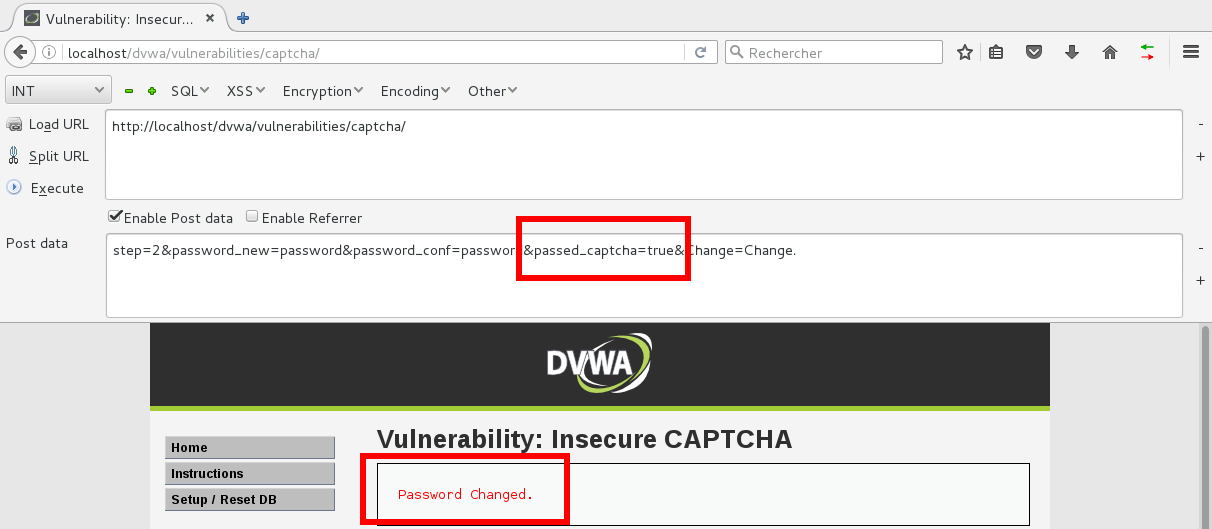
\includegraphics[scale=0.4]{images/captcha4.png}

\caption{Requête POST modifiant directement le mot de passe}
\label{captcha4}
\end{center}
\end{figure}

\subsubsection{Deuxième niveau}

\paragraph{Description de l'implémentation :}

Afin d'éviter l'accès direct à une troisième page nécessitant normalement la résolution d'un contrôle CAPTCHA en première page dont la vérification a lieu dans une deuxième page, les développeurs ont cette fois-ci géré la vérification du test sur la même page.

Cependant, en regardant le code source de la page HTML, on s'aperçoit que certains commentaires de développement n'ont pas été supprimés : 

\begin{quote}
\texttt{<!-- **DEV NOTE**   Response: 'hidd3n\_valu3'   \&\&   User-Agent: 'reCAPTCHA'   **/DEV NOTE** -->}
\end{quote}

On peut alors penser qu'il s'agit de valeurs permettant de tester la procédure du changement de mot de passe. Il est donc possible que ces valeurs puisse permettre d'outre-passer le contrôle CAPTCHA dans le script de modification du mot de passe. De plus, on peut légitimement penser que le champ "\texttt{Response: 'reCAPTCHA'}" correspond à la données de la requête POST "\texttt{recaptcha\_response\_field}" et que le champ \texttt{User-Agent: 'reCAPTCHA'} correspond à l'en-tête "\textit{User\_Agent}" de cette même requête.

On peut alors utiliser une nouvelle fois l'add-on "\href{https://addons.mozilla.org/fr/firefox/addon/tamper-data/}{\textit{Temper Data}}" de Firefox pour accéder à ces deux paramètres et les modifier (cf. figure \ref{captcha5}).

\begin{figure}[!h]
\begin{center}

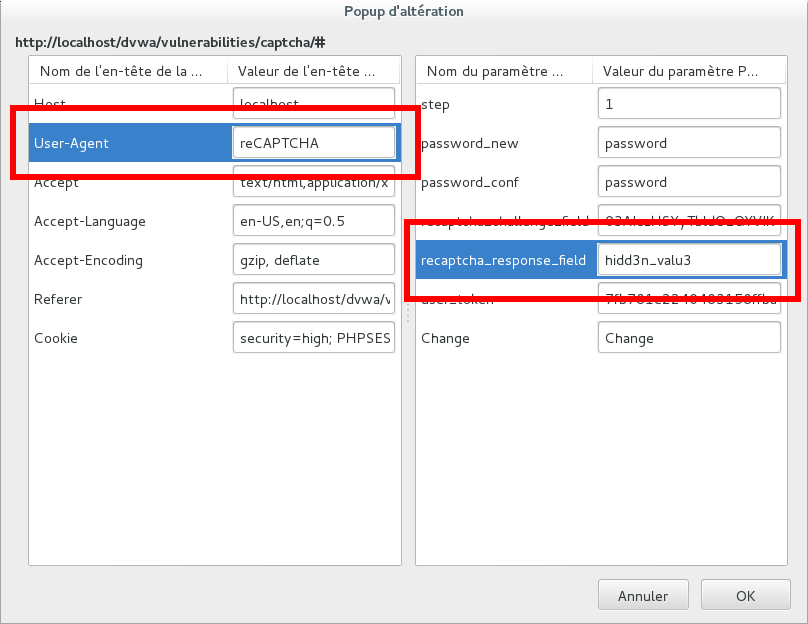
\includegraphics[scale=0.5]{images/captcha5.png}

\caption{Capture et modification de la requête POST}
\label{captcha5}
\end{center}
\end{figure}

On obtient alors bien une modification de mot de passe sans résoudre le contrôle CAPTCHA (cf. \ref{captcha6}). Une fois encore, cette création de requête POST peut être facilement automatisée, rendant pas là le test inefficace.\\

\begin{figure}[!h]
\begin{center}

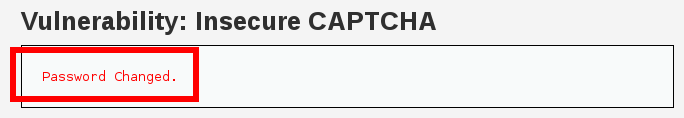
\includegraphics[scale=0.5]{images/captcha6.png}

\caption{Modification du mot de passe avec succès}
\label{captcha6}
\end{center}
\end{figure}

On voit donc que malgré l'utilisation d'une implémentation plus robuste, des erreurs de programmation de la part des développeurs peuvent mener à des failles allant à l'encontre même de ce qui était initialement souhaité. 

\subsubsection{Troisième niveau}

Dans ce troisième niveau implémenté, les commentaires et les portions de code utiles à des fins de test ont été supprimées. On se retrouve donc avec une implémentation beaucoup plus simple que les première proposées, reposant principalement sur la fonction \texttt{recaptcha\_check\_answer()} fournie par l'API reCAPTCHA et s'assurant du succès ou non au contrôle CAPTCHA.

Afin d'outre-passer les sécurités mises en place à ce niveau là, il serait nécessaire de se pencher vers les vulnérabilités permettant des résolutions automatiques par exemple, comme explicité dans la section \ref{desc_vul}.






\clearpage